\documentclass{standalone}
\usepackage{tikz}
\usetikzlibrary{patterns}
\usetikzlibrary{positioning}
\usetikzlibrary{patterns, positioning}
\usetikzlibrary{shapes.misc}
\usepackage[outline]{contour}
\contourlength{1.5pt} 
\usetikzlibrary{calc}
        \usepackage{relsize}
        \tikzset{fontscale/.style = {font=\relsize{#1}}}

\begin{document}
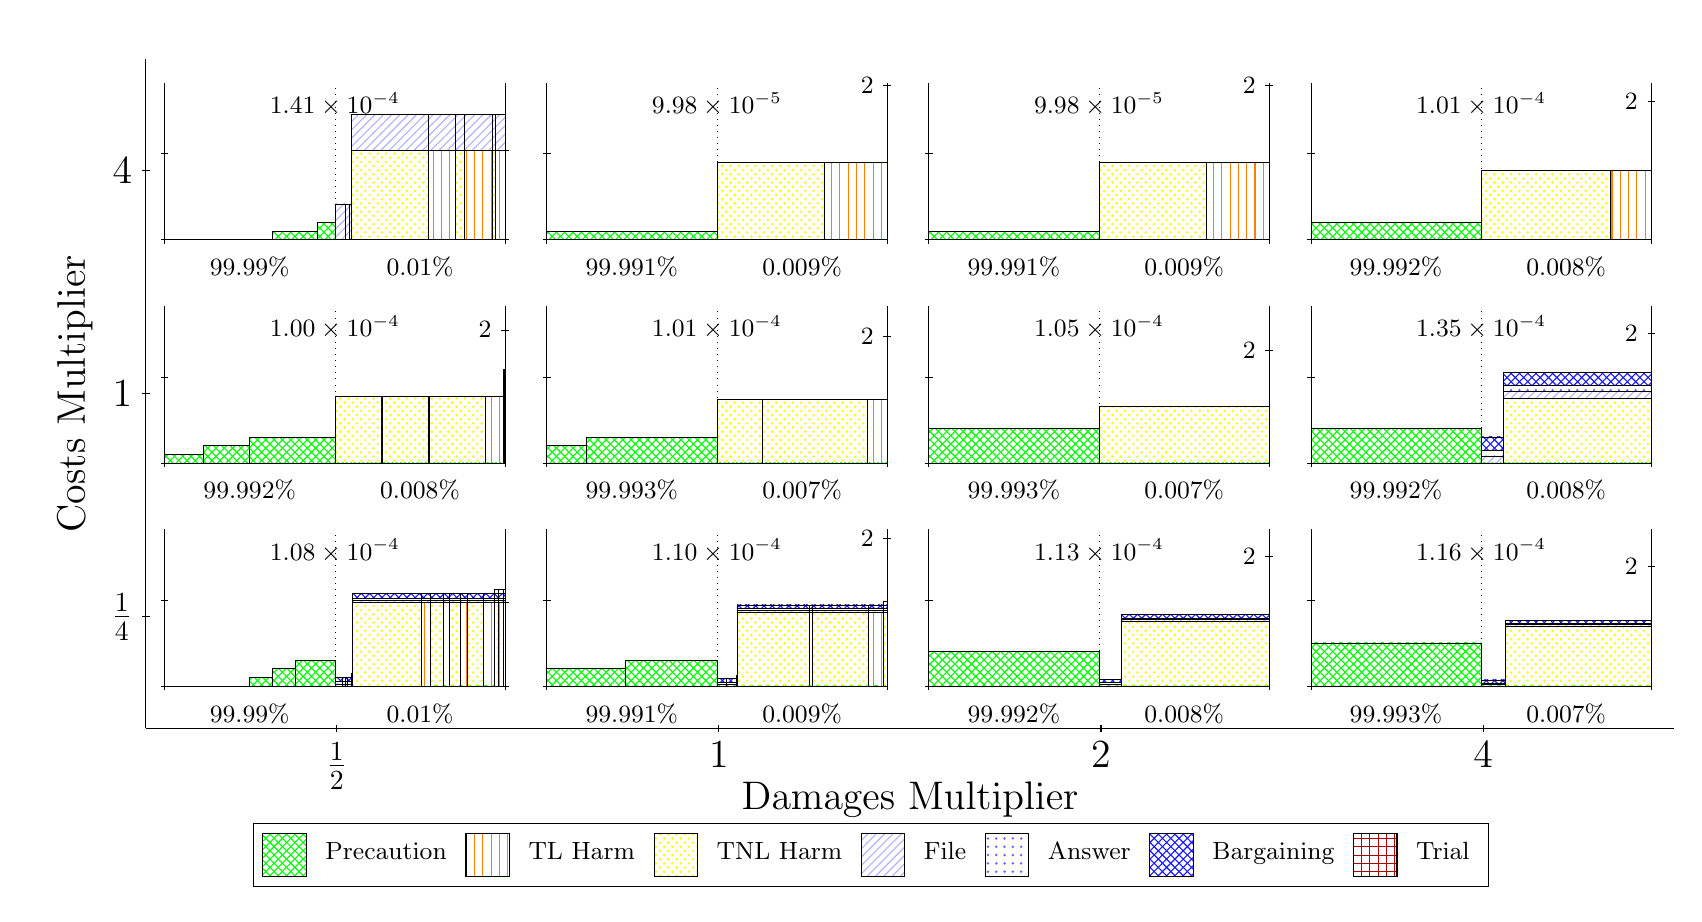
\begin{tikzpicture}
\clip(-0.5,-1.1) rectangle +(20.91,11);
\draw[black] (1,1) -- (1,9.5);
\node[rotate=90, fontscale=2, anchor=center] at (0.1, 5.25) {Costs Multiplier};
\draw[black] (0.95,2.4167) -- (1.05,2.4167);
\node[fontscale=2, anchor=east] at (0.95, 2.4167) {$\frac{1}{4}$};
\draw[black] (0.95,5.25) -- (1.05,5.25);
\node[fontscale=2, anchor=east] at (0.95, 5.25) {1};
\draw[black] (0.95,8.0833) -- (1.05,8.0833);
\node[fontscale=2, anchor=east] at (0.95, 8.0833) {4};

\draw[black] (1,1) -- (20.41,1);
\node[fontscale=2, anchor=center] at (10.705, 0.1) {Damages Multiplier};
\draw[black] (3.4263,0.95) -- (3.4263,1.05);
\node[fontscale=2, anchor=north] at (3.4263, 0.95) {$\frac{1}{2}$};
\draw[black] (8.2788,0.95) -- (8.2788,1.05);
\node[fontscale=2, anchor=north] at (8.2788, 0.95) {1};
\draw[black] (13.131,0.95) -- (13.131,1.05);
\node[fontscale=2, anchor=north] at (13.131, 0.95) {2};
\draw[black] (17.984,0.95) -- (17.984,1.05);
\node[fontscale=2, anchor=north] at (17.984, 0.95) {4};


\draw[pattern=crosshatch, pattern color=green,draw=black,very thin] (2.3197,1.54) rectangle (2.6114,1.6493);
\draw[pattern=crosshatch, pattern color=green,draw=black,very thin] (2.6114,1.54) rectangle (2.9037,1.7585);
\draw[pattern=crosshatch, pattern color=green,draw=black,very thin] (2.9037,1.54) rectangle (3.4013,1.8678);
\draw[pattern=north east lines, pattern color=blue!30,draw=black,very thin] (3.4013,1.54) rectangle (3.5003,1.5666);
\draw[pattern=dots,  pattern color=blue!60,draw=black,very thin] (3.4013,1.5666) rectangle (3.5003,1.5932);
\draw[pattern=crosshatch,      pattern color=blue!90,draw=black,very thin] (3.4013,1.5932) rectangle (3.5003,1.6465);
\draw[pattern=crosshatch, pattern color=green,draw=black,very thin] (3.5003,1.54) rectangle (3.5274,1.54);
\draw[pattern=north east lines, pattern color=blue!30,draw=black,very thin] (3.5003,1.54) rectangle (3.5274,1.5666);
\draw[pattern=dots,  pattern color=blue!60,draw=black,very thin] (3.5003,1.5666) rectangle (3.5274,1.5932);
\draw[pattern=crosshatch,      pattern color=blue!90,draw=black,very thin] (3.5003,1.5932) rectangle (3.5274,1.6465);
\draw[pattern=crosshatch, pattern color=green,draw=black,very thin] (3.5274,1.54) rectangle (3.5575,1.54);
\draw[pattern=north east lines, pattern color=blue!30,draw=black,very thin] (3.5274,1.54) rectangle (3.5575,1.5666);
\draw[pattern=dots,  pattern color=blue!60,draw=black,very thin] (3.5274,1.5666) rectangle (3.5575,1.5933);
\draw[pattern=crosshatch,      pattern color=blue!90,draw=black,very thin] (3.5274,1.5933) rectangle (3.5575,1.6465);
\draw[pattern=crosshatch, pattern color=green,draw=black,very thin] (3.5575,1.54) rectangle (3.6088,1.54);
\draw[pattern=north east lines, pattern color=blue!30,draw=black,very thin] (3.5575,1.54) rectangle (3.6088,1.5666);
\draw[pattern=dots,  pattern color=blue!60,draw=black,very thin] (3.5575,1.5666) rectangle (3.6088,1.5933);
\draw[pattern=crosshatch,      pattern color=blue!90,draw=black,very thin] (3.5575,1.5933) rectangle (3.6088,1.6465);
\draw[pattern=north east lines, pattern color=blue!30,draw=black,very thin] (3.6088,1.54) rectangle (3.6207,1.5666);
\draw[pattern=dots,  pattern color=blue!60,draw=black,very thin] (3.6088,1.5666) rectangle (3.6207,1.5932);
\draw[pattern=crosshatch,      pattern color=blue!90,draw=black,very thin] (3.6088,1.5932) rectangle (3.6207,1.6465);
\draw[pattern=grid,            pattern color=red!70!black,draw=black,very thin] (3.6088,1.6465) rectangle (3.6207,1.6997);
\draw[pattern=crosshatch, pattern color=green,draw=black,very thin] (3.6207,1.54) rectangle (3.6236,1.54);
\draw[pattern=north east lines, pattern color=blue!30,draw=black,very thin] (3.6207,1.54) rectangle (3.6236,1.5666);
\draw[pattern=dots,  pattern color=blue!60,draw=black,very thin] (3.6207,1.5666) rectangle (3.6236,1.5932);
\draw[pattern=crosshatch,      pattern color=blue!90,draw=black,very thin] (3.6207,1.5932) rectangle (3.6236,1.6465);
\draw[pattern=grid,            pattern color=red!70!black,draw=black,very thin] (3.6207,1.6465) rectangle (3.6236,1.6997);
\draw[pattern=crosshatch dots, pattern color=yellow,draw=black,very thin] (3.6236,1.54) rectangle (4.5028,2.6046);
\draw[pattern=north east lines, pattern color=blue!30,draw=black,very thin] (3.6236,2.6046) rectangle (4.5028,2.6312);
\draw[pattern=dots,  pattern color=blue!60,draw=black,very thin] (3.6236,2.6312) rectangle (4.5028,2.6579);
\draw[pattern=crosshatch,      pattern color=blue!90,draw=black,very thin] (3.6236,2.6579) rectangle (4.5028,2.7111);
\draw[pattern=vertical lines, pattern color=orange,draw=black,very thin] (4.5028,1.54) rectangle (4.6145,2.6046);
\draw[pattern=north east lines, pattern color=blue!30,draw=black,very thin] (4.5028,2.6046) rectangle (4.6145,2.6312);
\draw[pattern=dots,  pattern color=blue!60,draw=black,very thin] (4.5028,2.6312) rectangle (4.6145,2.6579);
\draw[pattern=crosshatch,      pattern color=blue!90,draw=black,very thin] (4.5028,2.6579) rectangle (4.6145,2.7111);
\draw[pattern=crosshatch, pattern color=green,draw=black,very thin] (4.6145,1.54) rectangle (4.7727,1.54);
\draw[pattern=crosshatch dots, pattern color=yellow,draw=black,very thin] (4.6145,1.54) rectangle (4.7727,2.6046);
\draw[pattern=north east lines, pattern color=blue!30,draw=black,very thin] (4.6145,2.6046) rectangle (4.7727,2.6313);
\draw[pattern=dots,  pattern color=blue!60,draw=black,very thin] (4.6145,2.6313) rectangle (4.7727,2.6579);
\draw[pattern=crosshatch,      pattern color=blue!90,draw=black,very thin] (4.6145,2.6579) rectangle (4.7727,2.7111);
\draw[pattern=crosshatch, pattern color=green,draw=black,very thin] (4.7727,1.54) rectangle (4.8564,1.54);
\draw[pattern=vertical lines, pattern color=orange,draw=black,very thin] (4.7727,1.54) rectangle (4.8564,2.6046);
\draw[pattern=north east lines, pattern color=blue!30,draw=black,very thin] (4.7727,2.6046) rectangle (4.8564,2.6313);
\draw[pattern=dots,  pattern color=blue!60,draw=black,very thin] (4.7727,2.6313) rectangle (4.8564,2.6579);
\draw[pattern=crosshatch,      pattern color=blue!90,draw=black,very thin] (4.7727,2.6579) rectangle (4.8564,2.7111);
\draw[pattern=crosshatch, pattern color=green,draw=black,very thin] (4.8564,1.54) rectangle (4.9929,1.54);
\draw[pattern=crosshatch dots, pattern color=yellow,draw=black,very thin] (4.8564,1.54) rectangle (4.9929,2.6046);
\draw[pattern=north east lines, pattern color=blue!30,draw=black,very thin] (4.8564,2.6046) rectangle (4.9929,2.6313);
\draw[pattern=dots,  pattern color=blue!60,draw=black,very thin] (4.8564,2.6313) rectangle (4.9929,2.6579);
\draw[pattern=crosshatch,      pattern color=blue!90,draw=black,very thin] (4.8564,2.6579) rectangle (4.9929,2.7111);
\draw[pattern=crosshatch, pattern color=green,draw=black,very thin] (4.9929,1.54) rectangle (5.0884,1.54);
\draw[pattern=vertical lines, pattern color=orange,draw=black,very thin] (4.9929,1.54) rectangle (5.0884,2.6046);
\draw[pattern=north east lines, pattern color=blue!30,draw=black,very thin] (4.9929,2.6046) rectangle (5.0884,2.6313);
\draw[pattern=dots,  pattern color=blue!60,draw=black,very thin] (4.9929,2.6313) rectangle (5.0884,2.6579);
\draw[pattern=crosshatch,      pattern color=blue!90,draw=black,very thin] (4.9929,2.6579) rectangle (5.0884,2.7111);
\draw[pattern=crosshatch, pattern color=green,draw=black,very thin] (5.0884,1.54) rectangle (5.2842,1.54);
\draw[pattern=crosshatch dots, pattern color=yellow,draw=black,very thin] (5.0884,1.54) rectangle (5.2842,2.6047);
\draw[pattern=north east lines, pattern color=blue!30,draw=black,very thin] (5.0884,2.6047) rectangle (5.2842,2.6313);
\draw[pattern=dots,  pattern color=blue!60,draw=black,very thin] (5.0884,2.6313) rectangle (5.2842,2.6579);
\draw[pattern=crosshatch,      pattern color=blue!90,draw=black,very thin] (5.0884,2.6579) rectangle (5.2842,2.7111);
\draw[pattern=crosshatch, pattern color=green,draw=black,very thin] (5.2842,1.54) rectangle (5.4202,1.54);
\draw[pattern=vertical lines, pattern color=orange,draw=black,very thin] (5.2842,1.54) rectangle (5.4202,2.6047);
\draw[pattern=north east lines, pattern color=blue!30,draw=black,very thin] (5.2842,2.6047) rectangle (5.4202,2.6313);
\draw[pattern=dots,  pattern color=blue!60,draw=black,very thin] (5.2842,2.6313) rectangle (5.4202,2.6579);
\draw[pattern=crosshatch,      pattern color=blue!90,draw=black,very thin] (5.2842,2.6579) rectangle (5.4202,2.7111);
\draw[pattern=crosshatch dots, pattern color=yellow,draw=black,very thin] (5.4202,1.54) rectangle (5.4798,2.6046);
\draw[pattern=north east lines, pattern color=blue!30,draw=black,very thin] (5.4202,2.6046) rectangle (5.4798,2.6312);
\draw[pattern=dots,  pattern color=blue!60,draw=black,very thin] (5.4202,2.6312) rectangle (5.4798,2.6579);
\draw[pattern=crosshatch,      pattern color=blue!90,draw=black,very thin] (5.4202,2.6579) rectangle (5.4798,2.7111);
\draw[pattern=grid,            pattern color=red!70!black,draw=black,very thin] (5.4202,2.7111) rectangle (5.4798,2.7643);
\draw[pattern=vertical lines, pattern color=orange,draw=black,very thin] (5.4798,1.54) rectangle (5.5394,2.6046);
\draw[pattern=north east lines, pattern color=blue!30,draw=black,very thin] (5.4798,2.6046) rectangle (5.5394,2.6312);
\draw[pattern=dots,  pattern color=blue!60,draw=black,very thin] (5.4798,2.6312) rectangle (5.5394,2.6579);
\draw[pattern=crosshatch,      pattern color=blue!90,draw=black,very thin] (5.4798,2.6579) rectangle (5.5394,2.7111);
\draw[pattern=grid,            pattern color=red!70!black,draw=black,very thin] (5.4798,2.7111) rectangle (5.5394,2.7643);
\draw[pattern=crosshatch, pattern color=green,draw=black,very thin] (5.5394,1.54) rectangle (5.5418,1.54);
\draw[pattern=crosshatch dots, pattern color=yellow,draw=black,very thin] (5.5394,1.54) rectangle (5.5418,2.6046);
\draw[pattern=north east lines, pattern color=blue!30,draw=black,very thin] (5.5394,2.6046) rectangle (5.5418,2.6313);
\draw[pattern=dots,  pattern color=blue!60,draw=black,very thin] (5.5394,2.6313) rectangle (5.5418,2.6579);
\draw[pattern=crosshatch,      pattern color=blue!90,draw=black,very thin] (5.5394,2.6579) rectangle (5.5418,2.7111);
\draw[pattern=grid,            pattern color=red!70!black,draw=black,very thin] (5.5394,2.7111) rectangle (5.5418,2.7643);
\draw[pattern=crosshatch, pattern color=green,draw=black,very thin] (5.5418,1.54) rectangle (5.5644,1.54);
\draw[pattern=vertical lines, pattern color=orange,draw=black,very thin] (5.5418,1.54) rectangle (5.5644,2.6046);
\draw[pattern=north east lines, pattern color=blue!30,draw=black,very thin] (5.5418,2.6046) rectangle (5.5644,2.6313);
\draw[pattern=dots,  pattern color=blue!60,draw=black,very thin] (5.5418,2.6313) rectangle (5.5644,2.6579);
\draw[pattern=crosshatch,      pattern color=blue!90,draw=black,very thin] (5.5418,2.6579) rectangle (5.5644,2.7111);
\draw[pattern=grid,            pattern color=red!70!black,draw=black,very thin] (5.5418,2.7111) rectangle (5.5644,2.7643);
\node[font=\small,text=black,anchor=north] at (3.4013, 3.5333) {$1.08\times 10^{-4}$};
\draw[black,very thin] (1.2381,1.54) -- (1.2381,3.5333);
\draw[black,very thin] (1.1881,1.54) -- (1.2881,1.54);
\node[font=\small,text=black, anchor=west] at (1.1881, 1.54) {};
\draw[black,very thin] (1.1881,2.6326) -- (1.2881,2.6326);
\node[font=\small,text=black, anchor=west] at (1.1881, 2.6326) {};

\draw[black,dotted,very thin] (3.4013,1.5998) -- (3.4013,3.4735);
\draw[black,very thin] (5.5644,1.54) -- (5.5644,3.5333);
\draw[black,very thin] (5.5144,1.54) -- (5.6144,1.54);
\node[font=\small,text=black, anchor=east] at (5.5144, 1.54) {\contour{white}{}};
\draw[black,very thin] (5.5144,2.6046) -- (5.6144,2.6046);
\node[font=\small,text=black, anchor=east] at (5.5144, 2.6046) {\contour{white}{}};

\draw[black,very thin] (1.2381,1.54) -- (5.5644,1.54);
\draw[black,very thin] (1.2381,1.49) -- (1.2381,1.59);
\node[font=\small,text=black, anchor=north] at (1.2381, 1.49) {};
\draw[black,very thin] (5.5644,1.49) -- (5.5644,1.59);
\node[font=\small,text=black, anchor=north] at (5.5644, 1.49) {};

\node[font=\small,text=black,anchor=south] at (2.3197, 0.94) {99.99\%};
\node[font=\small,text=black,anchor=south] at (4.4828, 0.94) {0.01\%};

\draw[pattern=crosshatch, pattern color=green,draw=black,very thin] (6.0906,1.54) rectangle (7.0842,1.7585);
\draw[pattern=crosshatch, pattern color=green,draw=black,very thin] (7.0842,1.54) rectangle (8.2538,1.8678);
\draw[pattern=crosshatch, pattern color=green,draw=black,very thin] (8.2538,1.54) rectangle (8.3696,1.54);
\draw[pattern=north east lines, pattern color=blue!30,draw=black,very thin] (8.2538,1.54) rectangle (8.3696,1.5634);
\draw[pattern=dots,  pattern color=blue!60,draw=black,very thin] (8.2538,1.5634) rectangle (8.3696,1.5868);
\draw[pattern=crosshatch,      pattern color=blue!90,draw=black,very thin] (8.2538,1.5868) rectangle (8.3696,1.6336);
\draw[pattern=crosshatch, pattern color=green,draw=black,very thin] (8.3696,1.54) rectangle (8.5008,1.54);
\draw[pattern=north east lines, pattern color=blue!30,draw=black,very thin] (8.3696,1.54) rectangle (8.5008,1.5634);
\draw[pattern=dots,  pattern color=blue!60,draw=black,very thin] (8.3696,1.5634) rectangle (8.5008,1.5868);
\draw[pattern=crosshatch,      pattern color=blue!90,draw=black,very thin] (8.3696,1.5868) rectangle (8.5008,1.6336);
\draw[pattern=crosshatch, pattern color=green,draw=black,very thin] (8.5008,1.54) rectangle (8.5064,1.54);
\draw[pattern=north east lines, pattern color=blue!30,draw=black,very thin] (8.5008,1.54) rectangle (8.5064,1.5634);
\draw[pattern=dots,  pattern color=blue!60,draw=black,very thin] (8.5008,1.5634) rectangle (8.5064,1.5868);
\draw[pattern=crosshatch,      pattern color=blue!90,draw=black,very thin] (8.5008,1.5868) rectangle (8.5064,1.6336);
\draw[pattern=grid,            pattern color=red!70!black,draw=black,very thin] (8.5008,1.6336) rectangle (8.5064,1.6804);
\draw[pattern=crosshatch, pattern color=green,draw=black,very thin] (8.5064,1.54) rectangle (9.4235,1.54);
\draw[pattern=crosshatch dots, pattern color=yellow,draw=black,very thin] (8.5064,1.54) rectangle (9.4235,2.476);
\draw[pattern=north east lines, pattern color=blue!30,draw=black,very thin] (8.5064,2.476) rectangle (9.4235,2.4994);
\draw[pattern=dots,  pattern color=blue!60,draw=black,very thin] (8.5064,2.4994) rectangle (9.4235,2.5228);
\draw[pattern=crosshatch,      pattern color=blue!90,draw=black,very thin] (8.5064,2.5228) rectangle (9.4235,2.5696);
\draw[pattern=crosshatch, pattern color=green,draw=black,very thin] (9.4235,1.54) rectangle (9.4684,1.54);
\draw[pattern=vertical lines, pattern color=orange,draw=black,very thin] (9.4235,1.54) rectangle (9.4684,2.476);
\draw[pattern=north east lines, pattern color=blue!30,draw=black,very thin] (9.4235,2.476) rectangle (9.4684,2.4994);
\draw[pattern=dots,  pattern color=blue!60,draw=black,very thin] (9.4235,2.4994) rectangle (9.4684,2.5228);
\draw[pattern=crosshatch,      pattern color=blue!90,draw=black,very thin] (9.4235,2.5228) rectangle (9.4684,2.5696);
\draw[pattern=crosshatch, pattern color=green,draw=black,very thin] (9.4684,1.54) rectangle (10.17,1.54);
\draw[pattern=crosshatch dots, pattern color=yellow,draw=black,very thin] (9.4684,1.54) rectangle (10.17,2.476);
\draw[pattern=north east lines, pattern color=blue!30,draw=black,very thin] (9.4684,2.476) rectangle (10.17,2.4994);
\draw[pattern=dots,  pattern color=blue!60,draw=black,very thin] (9.4684,2.4994) rectangle (10.17,2.5228);
\draw[pattern=crosshatch,      pattern color=blue!90,draw=black,very thin] (9.4684,2.5228) rectangle (10.17,2.5696);
\draw[pattern=crosshatch, pattern color=green,draw=black,very thin] (10.17,1.54) rectangle (10.372,1.54);
\draw[pattern=vertical lines, pattern color=orange,draw=black,very thin] (10.17,1.54) rectangle (10.372,2.476);
\draw[pattern=north east lines, pattern color=blue!30,draw=black,very thin] (10.17,2.476) rectangle (10.372,2.4994);
\draw[pattern=dots,  pattern color=blue!60,draw=black,very thin] (10.17,2.4994) rectangle (10.372,2.5228);
\draw[pattern=crosshatch,      pattern color=blue!90,draw=black,very thin] (10.17,2.5228) rectangle (10.372,2.5696);
\draw[pattern=crosshatch, pattern color=green,draw=black,very thin] (10.372,1.54) rectangle (10.417,1.54);
\draw[pattern=crosshatch dots, pattern color=yellow,draw=black,very thin] (10.372,1.54) rectangle (10.417,2.476);
\draw[pattern=north east lines, pattern color=blue!30,draw=black,very thin] (10.372,2.476) rectangle (10.417,2.4994);
\draw[pattern=dots,  pattern color=blue!60,draw=black,very thin] (10.372,2.4994) rectangle (10.417,2.5228);
\draw[pattern=crosshatch,      pattern color=blue!90,draw=black,very thin] (10.372,2.5228) rectangle (10.417,2.5696);
\draw[pattern=grid,            pattern color=red!70!black,draw=black,very thin] (10.372,2.5696) rectangle (10.417,2.6164);
\node[font=\small,text=black,anchor=north] at (8.2538, 3.5333) {$1.10\times 10^{-4}$};
\draw[black,very thin] (6.0906,1.54) -- (6.0906,3.5333);
\draw[black,very thin] (6.0406,1.54) -- (6.1406,1.54);
\node[font=\small,text=black, anchor=west] at (6.0406, 1.54) {};
\draw[black,very thin] (6.0406,2.6326) -- (6.1406,2.6326);
\node[font=\small,text=black, anchor=west] at (6.0406, 2.6326) {};

\draw[black,dotted,very thin] (8.2538,1.5998) -- (8.2538,3.4735);
\draw[black,very thin] (10.417,1.54) -- (10.417,3.5333);
\draw[black,very thin] (10.367,3.4119) -- (10.467,3.4119);
\node[font=\small,text=black, anchor=east] at (10.367, 3.4119) {\contour{white}{2}};

\draw[black,very thin] (6.0906,1.54) -- (10.417,1.54);
\draw[black,very thin] (6.0906,1.49) -- (6.0906,1.59);
\node[font=\small,text=black, anchor=north] at (6.0906, 1.49) {};
\draw[black,very thin] (10.417,1.49) -- (10.417,1.59);
\node[font=\small,text=black, anchor=north] at (10.417, 1.49) {};

\node[font=\small,text=black,anchor=south] at (7.1722, 0.94) {99.991\%};
\node[font=\small,text=black,anchor=south] at (9.3353, 0.94) {0.009\%};

\draw[pattern=crosshatch, pattern color=green,draw=black,very thin] (10.943,1.54) rectangle (13.106,1.9771);
\draw[pattern=crosshatch, pattern color=green,draw=black,very thin] (13.106,1.54) rectangle (13.394,1.54);
\draw[pattern=north east lines, pattern color=blue!30,draw=black,very thin] (13.106,1.54) rectangle (13.394,1.5606);
\draw[pattern=dots,  pattern color=blue!60,draw=black,very thin] (13.106,1.5606) rectangle (13.394,1.5812);
\draw[pattern=crosshatch,      pattern color=blue!90,draw=black,very thin] (13.106,1.5812) rectangle (13.394,1.6223);
\draw[pattern=crosshatch, pattern color=green,draw=black,very thin] (13.394,1.54) rectangle (15.269,1.54);
\draw[pattern=crosshatch dots, pattern color=yellow,draw=black,very thin] (13.394,1.54) rectangle (15.269,2.3631);
\draw[pattern=north east lines, pattern color=blue!30,draw=black,very thin] (13.394,2.3631) rectangle (15.269,2.3837);
\draw[pattern=dots,  pattern color=blue!60,draw=black,very thin] (13.394,2.3837) rectangle (15.269,2.4043);
\draw[pattern=crosshatch,      pattern color=blue!90,draw=black,very thin] (13.394,2.4043) rectangle (15.269,2.4454);
\node[font=\small,text=black,anchor=north] at (13.106, 3.5333) {$1.13\times 10^{-4}$};
\draw[black,very thin] (10.943,1.54) -- (10.943,3.5333);
\draw[black,very thin] (10.893,1.54) -- (10.993,1.54);
\node[font=\small,text=black, anchor=west] at (10.893, 1.54) {};
\draw[black,very thin] (10.893,2.6326) -- (10.993,2.6326);
\node[font=\small,text=black, anchor=west] at (10.893, 2.6326) {};

\draw[black,dotted,very thin] (13.106,1.5998) -- (13.106,3.4735);
\draw[black,very thin] (15.269,1.54) -- (15.269,3.5333);
\draw[black,very thin] (15.219,3.1861) -- (15.319,3.1861);
\node[font=\small,text=black, anchor=east] at (15.219, 3.1861) {\contour{white}{2}};

\draw[black,very thin] (10.943,1.54) -- (15.269,1.54);
\draw[black,very thin] (10.943,1.49) -- (10.943,1.59);
\node[font=\small,text=black, anchor=north] at (10.943, 1.49) {};
\draw[black,very thin] (15.269,1.49) -- (15.269,1.59);
\node[font=\small,text=black, anchor=north] at (15.269, 1.49) {};

\node[font=\small,text=black,anchor=south] at (12.025, 0.94) {99.992\%};
\node[font=\small,text=black,anchor=south] at (14.188, 0.94) {0.008\%};

\draw[pattern=crosshatch, pattern color=green,draw=black,very thin] (15.796,1.54) rectangle (17.959,2.0863);
\draw[pattern=crosshatch, pattern color=green,draw=black,very thin] (17.959,1.54) rectangle (18.271,1.54);
\draw[pattern=north east lines, pattern color=blue!30,draw=black,very thin] (17.959,1.54) rectangle (18.271,1.559);
\draw[pattern=dots,  pattern color=blue!60,draw=black,very thin] (17.959,1.559) rectangle (18.271,1.578);
\draw[pattern=crosshatch,      pattern color=blue!90,draw=black,very thin] (17.959,1.578) rectangle (18.271,1.6159);
\draw[pattern=crosshatch, pattern color=green,draw=black,very thin] (18.271,1.54) rectangle (20.122,1.54);
\draw[pattern=crosshatch dots, pattern color=yellow,draw=black,very thin] (18.271,1.54) rectangle (20.122,2.2984);
\draw[pattern=north east lines, pattern color=blue!30,draw=black,very thin] (18.271,2.2984) rectangle (20.122,2.3173);
\draw[pattern=dots,  pattern color=blue!60,draw=black,very thin] (18.271,2.3173) rectangle (20.122,2.3363);
\draw[pattern=crosshatch,      pattern color=blue!90,draw=black,very thin] (18.271,2.3363) rectangle (20.122,2.3742);
\node[font=\small,text=black,anchor=north] at (17.959, 3.5333) {$1.16\times 10^{-4}$};
\draw[black,very thin] (15.796,1.54) -- (15.796,3.5333);
\draw[black,very thin] (15.746,1.54) -- (15.846,1.54);
\node[font=\small,text=black, anchor=west] at (15.746, 1.54) {};
\draw[black,very thin] (15.746,2.6326) -- (15.846,2.6326);
\node[font=\small,text=black, anchor=west] at (15.746, 2.6326) {};

\draw[black,dotted,very thin] (17.959,1.5998) -- (17.959,3.4735);
\draw[black,very thin] (20.122,1.54) -- (20.122,3.5333);
\draw[black,very thin] (20.072,3.0567) -- (20.172,3.0567);
\node[font=\small,text=black, anchor=east] at (20.072, 3.0567) {\contour{white}{2}};

\draw[black,very thin] (15.796,1.54) -- (20.122,1.54);
\draw[black,very thin] (15.796,1.49) -- (15.796,1.59);
\node[font=\small,text=black, anchor=north] at (15.796, 1.49) {};
\draw[black,very thin] (20.122,1.49) -- (20.122,1.59);
\node[font=\small,text=black, anchor=north] at (20.122, 1.49) {};

\node[font=\small,text=black,anchor=south] at (16.877, 0.94) {99.993\%};
\node[font=\small,text=black,anchor=south] at (19.04, 0.94) {0.007\%};

\draw[pattern=crosshatch, pattern color=green,draw=black,very thin] (1.2381,4.3733) rectangle (1.7357,4.4826);
\draw[pattern=crosshatch, pattern color=green,draw=black,very thin] (1.7357,4.3733) rectangle (2.3197,4.5919);
\draw[pattern=crosshatch, pattern color=green,draw=black,very thin] (2.3197,4.3733) rectangle (3.4013,4.7011);
\draw[pattern=crosshatch, pattern color=green,draw=black,very thin] (3.4013,4.3733) rectangle (3.4036,4.3734);
\draw[pattern=north east lines, pattern color=blue!30,draw=black,very thin] (3.4013,4.3734) rectangle (3.4036,4.4578);
\draw[pattern=dots,  pattern color=blue!60,draw=black,very thin] (3.4013,4.4578) rectangle (3.4036,4.5422);
\draw[pattern=crosshatch,      pattern color=blue!90,draw=black,very thin] (3.4013,4.5422) rectangle (3.4036,4.7111);
\draw[pattern=crosshatch, pattern color=green,draw=black,very thin] (3.4036,4.3733) rectangle (3.9951,4.3733);
\draw[pattern=crosshatch dots, pattern color=yellow,draw=black,very thin] (3.4036,4.3733) rectangle (3.9951,5.2177);
\draw[pattern=crosshatch, pattern color=green,draw=black,very thin] (3.9951,4.3733) rectangle (3.9992,4.3733);
\draw[pattern=vertical lines, pattern color=orange,draw=black,very thin] (3.9951,4.3733) rectangle (3.9992,5.2177);
\draw[pattern=crosshatch, pattern color=green,draw=black,very thin] (3.9992,4.3733) rectangle (4.5899,4.3734);
\draw[pattern=crosshatch dots, pattern color=yellow,draw=black,very thin] (3.9992,4.3734) rectangle (4.5899,5.2177);
\draw[pattern=crosshatch, pattern color=green,draw=black,very thin] (4.5899,4.3733) rectangle (4.6053,4.3734);
\draw[pattern=vertical lines, pattern color=orange,draw=black,very thin] (4.5899,4.3734) rectangle (4.6053,5.2177);
\draw[pattern=crosshatch, pattern color=green,draw=black,very thin] (4.6053,4.3733) rectangle (5.3137,4.3734);
\draw[pattern=crosshatch dots, pattern color=yellow,draw=black,very thin] (4.6053,4.3734) rectangle (5.3137,5.2177);
\draw[pattern=crosshatch, pattern color=green,draw=black,very thin] (5.3137,4.3733) rectangle (5.546,4.3734);
\draw[pattern=vertical lines, pattern color=orange,draw=black,very thin] (5.3137,4.3734) rectangle (5.546,5.2177);
\draw[pattern=crosshatch, pattern color=green,draw=black,very thin] (5.546,4.3733) rectangle (5.5571,4.3734);
\draw[pattern=crosshatch dots, pattern color=yellow,draw=black,very thin] (5.546,4.3734) rectangle (5.5571,5.2177);
\draw[pattern=north east lines, pattern color=blue!30,draw=black,very thin] (5.546,5.2177) rectangle (5.5571,5.3021);
\draw[pattern=dots,  pattern color=blue!60,draw=black,very thin] (5.546,5.3021) rectangle (5.5571,5.3866);
\draw[pattern=crosshatch,      pattern color=blue!90,draw=black,very thin] (5.546,5.3866) rectangle (5.5571,5.5554);
\draw[pattern=crosshatch, pattern color=green,draw=black,very thin] (5.5571,4.3733) rectangle (5.5644,4.3734);
\draw[pattern=vertical lines, pattern color=orange,draw=black,very thin] (5.5571,4.3734) rectangle (5.5644,5.2177);
\draw[pattern=north east lines, pattern color=blue!30,draw=black,very thin] (5.5571,5.2177) rectangle (5.5644,5.3021);
\draw[pattern=dots,  pattern color=blue!60,draw=black,very thin] (5.5571,5.3021) rectangle (5.5644,5.3866);
\draw[pattern=crosshatch,      pattern color=blue!90,draw=black,very thin] (5.5571,5.3866) rectangle (5.5644,5.5554);
\node[font=\small,text=black,anchor=north] at (3.4013, 6.3667) {$1.00\times 10^{-4}$};
\draw[black,very thin] (1.2381,4.3733) -- (1.2381,6.3667);
\draw[black,very thin] (1.1881,4.3733) -- (1.2881,4.3733);
\node[font=\small,text=black, anchor=west] at (1.1881, 4.3733) {};
\draw[black,very thin] (1.1881,5.466) -- (1.2881,5.466);
\node[font=\small,text=black, anchor=west] at (1.1881, 5.466) {};

\draw[black,dotted,very thin] (3.4013,4.4331) -- (3.4013,6.3069);
\draw[black,very thin] (5.5644,4.3733) -- (5.5644,6.3667);
\draw[black,very thin] (5.5144,6.062) -- (5.6144,6.062);
\node[font=\small,text=black, anchor=east] at (5.5144, 6.062) {\contour{white}{2}};

\draw[black,very thin] (1.2381,4.3733) -- (5.5644,4.3733);
\draw[black,very thin] (1.2381,4.3233) -- (1.2381,4.4233);
\node[font=\small,text=black, anchor=north] at (1.2381, 4.3233) {};
\draw[black,very thin] (5.5644,4.3233) -- (5.5644,4.4233);
\node[font=\small,text=black, anchor=north] at (5.5644, 4.3233) {};

\node[font=\small,text=black,anchor=south] at (2.3197, 3.7733) {99.992\%};
\node[font=\small,text=black,anchor=south] at (4.4828, 3.7733) {0.008\%};

\draw[pattern=crosshatch, pattern color=green,draw=black,very thin] (6.0906,4.3733) rectangle (6.5882,4.5919);
\draw[pattern=crosshatch, pattern color=green,draw=black,very thin] (6.5882,4.3733) rectangle (8.2538,4.7011);
\draw[pattern=crosshatch, pattern color=green,draw=black,very thin] (8.2538,4.3733) rectangle (8.8327,4.3733);
\draw[pattern=crosshatch dots, pattern color=yellow,draw=black,very thin] (8.2538,4.3733) rectangle (8.8327,5.1789);
\draw[pattern=crosshatch, pattern color=green,draw=black,very thin] (8.8327,4.3733) rectangle (8.8334,4.3733);
\draw[pattern=vertical lines, pattern color=orange,draw=black,very thin] (8.8327,4.3733) rectangle (8.8334,5.1789);
\draw[pattern=crosshatch, pattern color=green,draw=black,very thin] (8.8334,4.3733) rectangle (10.168,4.3734);
\draw[pattern=crosshatch dots, pattern color=yellow,draw=black,very thin] (8.8334,4.3734) rectangle (10.168,5.1789);
\draw[pattern=crosshatch, pattern color=green,draw=black,very thin] (10.168,4.3733) rectangle (10.417,4.3734);
\draw[pattern=vertical lines, pattern color=orange,draw=black,very thin] (10.168,4.3734) rectangle (10.417,5.1789);
\node[font=\small,text=black,anchor=north] at (8.2538, 6.3667) {$1.01\times 10^{-4}$};
\draw[black,very thin] (6.0906,4.3733) -- (6.0906,6.3667);
\draw[black,very thin] (6.0406,4.3733) -- (6.1406,4.3733);
\node[font=\small,text=black, anchor=west] at (6.0406, 4.3733) {};
\draw[black,very thin] (6.0406,5.466) -- (6.1406,5.466);
\node[font=\small,text=black, anchor=west] at (6.0406, 5.466) {};

\draw[black,dotted,very thin] (8.2538,4.4331) -- (8.2538,6.3069);
\draw[black,very thin] (10.417,4.3733) -- (10.417,6.3667);
\draw[black,very thin] (10.367,5.9845) -- (10.467,5.9845);
\node[font=\small,text=black, anchor=east] at (10.367, 5.9845) {\contour{white}{2}};

\draw[black,very thin] (6.0906,4.3733) -- (10.417,4.3733);
\draw[black,very thin] (6.0906,4.3233) -- (6.0906,4.4233);
\node[font=\small,text=black, anchor=north] at (6.0906, 4.3233) {};
\draw[black,very thin] (10.417,4.3233) -- (10.417,4.4233);
\node[font=\small,text=black, anchor=north] at (10.417, 4.3233) {};

\node[font=\small,text=black,anchor=south] at (7.1722, 3.7733) {99.993\%};
\node[font=\small,text=black,anchor=south] at (9.3353, 3.7733) {0.007\%};

\draw[pattern=crosshatch, pattern color=green,draw=black,very thin] (10.943,4.3733) rectangle (13.106,4.8104);
\draw[pattern=crosshatch, pattern color=green,draw=black,very thin] (13.106,4.3733) rectangle (15.269,4.3734);
\draw[pattern=crosshatch dots, pattern color=yellow,draw=black,very thin] (13.106,4.3734) rectangle (15.269,5.0871);
\node[font=\small,text=black,anchor=north] at (13.106, 6.3667) {$1.05\times 10^{-4}$};
\draw[black,very thin] (10.943,4.3733) -- (10.943,6.3667);
\draw[black,very thin] (10.893,4.3733) -- (10.993,4.3733);
\node[font=\small,text=black, anchor=west] at (10.893, 4.3733) {};
\draw[black,very thin] (10.893,5.466) -- (10.993,5.466);
\node[font=\small,text=black, anchor=west] at (10.893, 5.466) {};

\draw[black,dotted,very thin] (13.106,4.4331) -- (13.106,6.3069);
\draw[black,very thin] (15.269,4.3733) -- (15.269,6.3667);
\draw[black,very thin] (15.219,5.8009) -- (15.319,5.8009);
\node[font=\small,text=black, anchor=east] at (15.219, 5.8009) {\contour{white}{2}};

\draw[black,very thin] (10.943,4.3733) -- (15.269,4.3733);
\draw[black,very thin] (10.943,4.3233) -- (10.943,4.4233);
\node[font=\small,text=black, anchor=north] at (10.943, 4.3233) {};
\draw[black,very thin] (15.269,4.3233) -- (15.269,4.4233);
\node[font=\small,text=black, anchor=north] at (15.269, 4.3233) {};

\node[font=\small,text=black,anchor=south] at (12.025, 3.7733) {99.993\%};
\node[font=\small,text=black,anchor=south] at (14.188, 3.7733) {0.007\%};

\draw[pattern=crosshatch, pattern color=green,draw=black,very thin] (15.796,4.3733) rectangle (17.959,4.8104);
\draw[pattern=crosshatch, pattern color=green,draw=black,very thin] (17.959,4.3733) rectangle (18.246,4.3734);
\draw[pattern=north east lines, pattern color=blue!30,draw=black,very thin] (17.959,4.3734) rectangle (18.246,4.4557);
\draw[pattern=dots,  pattern color=blue!60,draw=black,very thin] (17.959,4.4557) rectangle (18.246,4.538);
\draw[pattern=crosshatch,      pattern color=blue!90,draw=black,very thin] (17.959,4.538) rectangle (18.246,4.7026);
\draw[pattern=crosshatch, pattern color=green,draw=black,very thin] (18.246,4.3733) rectangle (20.122,4.3734);
\draw[pattern=crosshatch dots, pattern color=yellow,draw=black,very thin] (18.246,4.3734) rectangle (20.122,5.1964);
\draw[pattern=north east lines, pattern color=blue!30,draw=black,very thin] (18.246,5.1964) rectangle (20.122,5.2787);
\draw[pattern=dots,  pattern color=blue!60,draw=black,very thin] (18.246,5.2787) rectangle (20.122,5.3611);
\draw[pattern=crosshatch,      pattern color=blue!90,draw=black,very thin] (18.246,5.3611) rectangle (20.122,5.5257);
\node[font=\small,text=black,anchor=north] at (17.959, 6.3667) {$1.35\times 10^{-4}$};
\draw[black,very thin] (15.796,4.3733) -- (15.796,6.3667);
\draw[black,very thin] (15.746,4.3733) -- (15.846,4.3733);
\node[font=\small,text=black, anchor=west] at (15.746, 4.3733) {};
\draw[black,very thin] (15.746,5.466) -- (15.846,5.466);
\node[font=\small,text=black, anchor=west] at (15.746, 5.466) {};

\draw[black,dotted,very thin] (17.959,4.4331) -- (17.959,6.3069);
\draw[black,very thin] (20.122,4.3733) -- (20.122,6.3667);
\draw[black,very thin] (20.072,6.0195) -- (20.172,6.0195);
\node[font=\small,text=black, anchor=east] at (20.072, 6.0195) {\contour{white}{2}};

\draw[black,very thin] (15.796,4.3733) -- (20.122,4.3733);
\draw[black,very thin] (15.796,4.3233) -- (15.796,4.4233);
\node[font=\small,text=black, anchor=north] at (15.796, 4.3233) {};
\draw[black,very thin] (20.122,4.3233) -- (20.122,4.4233);
\node[font=\small,text=black, anchor=north] at (20.122, 4.3233) {};

\node[font=\small,text=black,anchor=south] at (16.877, 3.7733) {99.992\%};
\node[font=\small,text=black,anchor=south] at (19.04, 3.7733) {0.008\%};

\draw[pattern=crosshatch, pattern color=green,draw=black,very thin] (2.6114,7.2067) rectangle (3.1788,7.3159);
\draw[pattern=crosshatch, pattern color=green,draw=black,very thin] (3.1788,7.2067) rectangle (3.4013,7.4252);
\draw[pattern=north east lines, pattern color=blue!30,draw=black,very thin] (3.4013,7.2067) rectangle (3.533,7.6623);
\draw[pattern=crosshatch, pattern color=green,draw=black,very thin] (3.533,7.2067) rectangle (3.5875,7.2067);
\draw[pattern=north east lines, pattern color=blue!30,draw=black,very thin] (3.533,7.2067) rectangle (3.5875,7.6623);
\draw[pattern=crosshatch, pattern color=green,draw=black,very thin] (3.5875,7.2067) rectangle (3.6089,7.2067);
\draw[pattern=north east lines, pattern color=blue!30,draw=black,very thin] (3.5875,7.2067) rectangle (3.6089,7.6623);
\draw[pattern=crosshatch dots, pattern color=yellow,draw=black,very thin] (3.6089,7.2067) rectangle (4.5885,8.3457);
\draw[pattern=north east lines, pattern color=blue!30,draw=black,very thin] (3.6089,8.3457) rectangle (4.5885,8.8013);
\draw[pattern=vertical lines, pattern color=orange,draw=black,very thin] (4.5885,7.2067) rectangle (4.9263,8.3457);
\draw[pattern=north east lines, pattern color=blue!30,draw=black,very thin] (4.5885,8.3457) rectangle (4.9263,8.8013);
\draw[pattern=crosshatch, pattern color=green,draw=black,very thin] (4.9263,7.2067) rectangle (5.0456,7.2067);
\draw[pattern=crosshatch dots, pattern color=yellow,draw=black,very thin] (4.9263,7.2067) rectangle (5.0456,8.3457);
\draw[pattern=north east lines, pattern color=blue!30,draw=black,very thin] (4.9263,8.3457) rectangle (5.0456,8.8013);
\draw[pattern=crosshatch, pattern color=green,draw=black,very thin] (5.0456,7.2067) rectangle (5.4043,7.2067);
\draw[pattern=vertical lines, pattern color=orange,draw=black,very thin] (5.0456,7.2067) rectangle (5.4043,8.3457);
\draw[pattern=north east lines, pattern color=blue!30,draw=black,very thin] (5.0456,8.3457) rectangle (5.4043,8.8013);
\draw[pattern=crosshatch, pattern color=green,draw=black,very thin] (5.4043,7.2067) rectangle (5.435,7.2067);
\draw[pattern=crosshatch dots, pattern color=yellow,draw=black,very thin] (5.4043,7.2067) rectangle (5.435,8.3457);
\draw[pattern=north east lines, pattern color=blue!30,draw=black,very thin] (5.4043,8.3457) rectangle (5.435,8.8013);
\draw[pattern=crosshatch, pattern color=green,draw=black,very thin] (5.435,7.2067) rectangle (5.5644,7.2067);
\draw[pattern=vertical lines, pattern color=orange,draw=black,very thin] (5.435,7.2067) rectangle (5.5644,8.3457);
\draw[pattern=north east lines, pattern color=blue!30,draw=black,very thin] (5.435,8.3457) rectangle (5.5644,8.8013);
\node[font=\small,text=black,anchor=north] at (3.4013, 9.2) {$1.41\times 10^{-4}$};
\draw[black,very thin] (1.2381,7.2067) -- (1.2381,9.2);
\draw[black,very thin] (1.1881,7.2067) -- (1.2881,7.2067);
\node[font=\small,text=black, anchor=west] at (1.1881, 7.2067) {};
\draw[black,very thin] (1.1881,8.2993) -- (1.2881,8.2993);
\node[font=\small,text=black, anchor=west] at (1.1881, 8.2993) {};

\draw[black,dotted,very thin] (3.4013,7.2665) -- (3.4013,9.1402);
\draw[black,very thin] (5.5644,7.2067) -- (5.5644,9.2);
\draw[black,very thin] (5.5144,7.2067) -- (5.6144,7.2067);
\node[font=\small,text=black, anchor=east] at (5.5144, 7.2067) {\contour{white}{}};
\draw[black,very thin] (5.5144,8.3457) -- (5.6144,8.3457);
\node[font=\small,text=black, anchor=east] at (5.5144, 8.3457) {\contour{white}{}};

\draw[black,very thin] (1.2381,7.2067) -- (5.5644,7.2067);
\draw[black,very thin] (1.2381,7.1567) -- (1.2381,7.2567);
\node[font=\small,text=black, anchor=north] at (1.2381, 7.1567) {};
\draw[black,very thin] (5.5644,7.1567) -- (5.5644,7.2567);
\node[font=\small,text=black, anchor=north] at (5.5644, 7.1567) {};

\node[font=\small,text=black,anchor=south] at (2.3197, 6.6067) {99.99\%};
\node[font=\small,text=black,anchor=south] at (4.4828, 6.6067) {0.01\%};

\draw[pattern=crosshatch, pattern color=green,draw=black,very thin] (6.0906,7.2067) rectangle (8.2538,7.3159);
\draw[pattern=crosshatch, pattern color=green,draw=black,very thin] (8.2538,7.2067) rectangle (9.6129,7.2067);
\draw[pattern=crosshatch dots, pattern color=yellow,draw=black,very thin] (8.2538,7.2067) rectangle (9.6129,8.1879);
\draw[pattern=crosshatch, pattern color=green,draw=black,very thin] (9.6129,7.2067) rectangle (10.417,7.2067);
\draw[pattern=vertical lines, pattern color=orange,draw=black,very thin] (9.6129,7.2067) rectangle (10.417,8.1879);
\node[font=\small,text=black,anchor=north] at (8.2538, 9.2) {$9.98\times 10^{-5}$};
\draw[black,very thin] (6.0906,7.2067) -- (6.0906,9.2);
\draw[black,very thin] (6.0406,7.2067) -- (6.1406,7.2067);
\node[font=\small,text=black, anchor=west] at (6.0406, 7.2067) {};
\draw[black,very thin] (6.0406,8.2993) -- (6.1406,8.2993);
\node[font=\small,text=black, anchor=west] at (6.0406, 8.2993) {};

\draw[black,dotted,very thin] (8.2538,7.2665) -- (8.2538,9.1402);
\draw[black,very thin] (10.417,7.2067) -- (10.417,9.2);
\draw[black,very thin] (10.367,9.169) -- (10.467,9.169);
\node[font=\small,text=black, anchor=east] at (10.367, 9.169) {\contour{white}{2}};

\draw[black,very thin] (6.0906,7.2067) -- (10.417,7.2067);
\draw[black,very thin] (6.0906,7.1567) -- (6.0906,7.2567);
\node[font=\small,text=black, anchor=north] at (6.0906, 7.1567) {};
\draw[black,very thin] (10.417,7.1567) -- (10.417,7.2567);
\node[font=\small,text=black, anchor=north] at (10.417, 7.1567) {};

\node[font=\small,text=black,anchor=south] at (7.1722, 6.6067) {99.991\%};
\node[font=\small,text=black,anchor=south] at (9.3353, 6.6067) {0.009\%};

\draw[pattern=crosshatch, pattern color=green,draw=black,very thin] (10.943,7.2067) rectangle (13.106,7.3159);
\draw[pattern=crosshatch, pattern color=green,draw=black,very thin] (13.106,7.2067) rectangle (14.465,7.2067);
\draw[pattern=crosshatch dots, pattern color=yellow,draw=black,very thin] (13.106,7.2067) rectangle (14.465,8.1879);
\draw[pattern=crosshatch, pattern color=green,draw=black,very thin] (14.465,7.2067) rectangle (15.269,7.2067);
\draw[pattern=vertical lines, pattern color=orange,draw=black,very thin] (14.465,7.2067) rectangle (15.269,8.1879);
\node[font=\small,text=black,anchor=north] at (13.106, 9.2) {$9.98\times 10^{-5}$};
\draw[black,very thin] (10.943,7.2067) -- (10.943,9.2);
\draw[black,very thin] (10.893,7.2067) -- (10.993,7.2067);
\node[font=\small,text=black, anchor=west] at (10.893, 7.2067) {};
\draw[black,very thin] (10.893,8.2993) -- (10.993,8.2993);
\node[font=\small,text=black, anchor=west] at (10.893, 8.2993) {};

\draw[black,dotted,very thin] (13.106,7.2665) -- (13.106,9.1402);
\draw[black,very thin] (15.269,7.2067) -- (15.269,9.2);
\draw[black,very thin] (15.219,9.169) -- (15.319,9.169);
\node[font=\small,text=black, anchor=east] at (15.219, 9.169) {\contour{white}{2}};

\draw[black,very thin] (10.943,7.2067) -- (15.269,7.2067);
\draw[black,very thin] (10.943,7.1567) -- (10.943,7.2567);
\node[font=\small,text=black, anchor=north] at (10.943, 7.1567) {};
\draw[black,very thin] (15.269,7.1567) -- (15.269,7.2567);
\node[font=\small,text=black, anchor=north] at (15.269, 7.1567) {};

\node[font=\small,text=black,anchor=south] at (12.025, 6.6067) {99.991\%};
\node[font=\small,text=black,anchor=south] at (14.188, 6.6067) {0.009\%};

\draw[pattern=crosshatch, pattern color=green,draw=black,very thin] (15.796,7.2067) rectangle (17.959,7.4252);
\draw[pattern=crosshatch, pattern color=green,draw=black,very thin] (17.959,7.2067) rectangle (19.595,7.2067);
\draw[pattern=crosshatch dots, pattern color=yellow,draw=black,very thin] (17.959,7.2067) rectangle (19.595,8.0872);
\draw[pattern=crosshatch, pattern color=green,draw=black,very thin] (19.595,7.2067) rectangle (20.122,7.2067);
\draw[pattern=vertical lines, pattern color=orange,draw=black,very thin] (19.595,7.2067) rectangle (20.122,8.0872);
\node[font=\small,text=black,anchor=north] at (17.959, 9.2) {$1.01\times 10^{-4}$};
\draw[black,very thin] (15.796,7.2067) -- (15.796,9.2);
\draw[black,very thin] (15.746,7.2067) -- (15.846,7.2067);
\node[font=\small,text=black, anchor=west] at (15.746, 7.2067) {};
\draw[black,very thin] (15.746,8.2993) -- (15.846,8.2993);
\node[font=\small,text=black, anchor=west] at (15.746, 8.2993) {};

\draw[black,dotted,very thin] (17.959,7.2665) -- (17.959,9.1402);
\draw[black,very thin] (20.122,7.2067) -- (20.122,9.2);
\draw[black,very thin] (20.072,8.9677) -- (20.172,8.9677);
\node[font=\small,text=black, anchor=east] at (20.072, 8.9677) {\contour{white}{2}};

\draw[black,very thin] (15.796,7.2067) -- (20.122,7.2067);
\draw[black,very thin] (15.796,7.1567) -- (15.796,7.2567);
\node[font=\small,text=black, anchor=north] at (15.796, 7.1567) {};
\draw[black,very thin] (20.122,7.1567) -- (20.122,7.2567);
\node[font=\small,text=black, anchor=north] at (20.122, 7.1567) {};

\node[font=\small,text=black,anchor=south] at (16.877, 6.6067) {99.992\%};
\node[font=\small,text=black,anchor=south] at (19.04, 6.6067) {0.008\%};

\coordinate (LegendAnchor) at (10.205000000000002,0);
\begin{scope}[align=center]
\matrix[scale=0.6,draw=black,below=0.2cm of LegendAnchor,nodes={draw},column sep=0.12cm]{
\node[rectangle,draw,minimum width=0.55cm,minimum height=0.55cm,pattern=crosshatch, pattern color=green]{}; &
        \node[draw=none,font=\small]{Precaution}; &
\node[rectangle,draw,minimum width=0.55cm,minimum height=0.55cm,pattern=vertical lines, pattern color=orange]{}; &
        \node[draw=none,font=\small]{TL Harm}; &
\node[rectangle,draw,minimum width=0.55cm,minimum height=0.55cm,pattern=crosshatch dots, pattern color=yellow]{}; &
        \node[draw=none,font=\small]{TNL Harm}; &
\node[rectangle,draw,minimum width=0.55cm,minimum height=0.55cm,pattern=north east lines, pattern color=blue!30]{}; &
        \node[draw=none,font=\small]{File}; &
\node[rectangle,draw,minimum width=0.55cm,minimum height=0.55cm,pattern=dots, pattern color=blue!60]{}; &
        \node[draw=none,font=\small]{Answer}; &
\node[rectangle,draw,minimum width=0.55cm,minimum height=0.55cm,pattern=crosshatch, pattern color=blue!90]{}; &
        \node[draw=none,font=\small]{Bargaining}; &
\node[rectangle,draw,minimum width=0.55cm,minimum height=0.55cm,pattern=grid, pattern color=red!70!black]{}; &
        \node[draw=none,font=\small]{Trial}; \\
};\end{scope}

\end{tikzpicture}
\end{document}